\chapter{State estimation for legged robots: a literature review}
%
The field of state estimation for autonomous systems is at the frontier between many fields including automation, probability theory, nonlinear estimation etc.
The general aim is to design and implement computationally tractable algorithms using noisy causal sensor measurements that can be embedded in feedback-controlled systems.
With the advent of digital computers and the theoretical breakthroughs of Kalman \cite{kalman1960new} among others, a vast family of observers has been developed 
\cite{fujii2013extended, wan2001unscented} [cite Information filter]. Applications range the full scope of autonomous systems from spacecraft guidance \cite{mcgee1985discovery} 
to autonomous underwater vehicle navigation \cite{leonard2016autonomous}. Each application has its own specific sets of requirements, depending on the physical
nature of the system and its environment, available sensors, and embedded computation power. Legged robots in particular require a high frequency (kHz) 
and low latency estimates owing to the inherent instability of the dynamical system. Moreover, they interact with the environment through 
intermittent contacts to move around, which requires to plan in advance the motion using Model Predictive Control (MPC). These tight requirements 
have given birth to a wealth of research works that are now commonly used in commercial products \cite{hutter2016anymal}.

We will focus our review on works applying state estimation theory on legged robots, which include mainly quadrupeds and humanoid robots. The first part will 
be centered around proprioceptive estimation of the robot's base. We will then examine the estimation of centroidal quantities. The use of exteroceptive sensors
to obtain information from the robot environment will then be described. Finally, we will see that a new class of optimization-based estimator is a promising alternative
to filtering-based methods.

\section{Definitions}
\label{sec:def}
Let's first introduce terms and key concepts that are commonly used in the legged robot estimation literature.

\textit{Legged robot} are poly-articulated systems that use a set of end-effectors (commonly referred to as feet whatever their nature) to move their main body
by pushing on its environment. The kinematic chain of the robot is modeled as a graph composed of fixed shape segments (aka. links) 
linked together by articulations (aka. joints). Joints come in various forms (revolute, prismatic, ball...) and can be actuated or not.
The \textit{base} refers to a reference frame rigidly attached to the main body of the robot (often the trunk for quadrupeds and the pelvis for humanoids). 
We are most often interested in the estimation of the position, velocity, and orientation of this frame with regard to an inertial \textit{world} frame, which is called the \textit{base state}. 
An example of these frames is given for the Solo robot in \figRef{{fig:solo_frames}}.
This estimation is the main focus in most of legged robot estimation literature. In fact, knowing the base and other quantities directly measurable (such as joint angles), 
and assuming a perfect robot kinematic model, the state of any part of the poly-articulated system can be recovered using forward kinematics. Rigid body algorithms
\cite{featherstone2014rigid} provide methods to efficiently compute the center of mass, linear and angular momentum of the  poly-articulated systems. These computations
are again based on the robot kinematic model as well as the segments inertia, which we together call the $kinodynamic$ robot model. This model is often 
found in urdf files (Unified Robot Description Format) which are generated via CAD models.

The \textit{centroidal state} refer to the center of mass, angular momentum, and their derivatives. The center 
of mass (barycenter of the robot segment masses) is a virtual point that is the main control variable for locomotion. 
%Centroidal estimators fuse the robot kinematic model, which is often assumed to be biased, with various dynamical models of the system. 

\textit{Proprioceptive} sensors measure values about the internal state of the robot. For legged robots, they include joint encoders, strain gauges measuring 
either joint torques or end-effector torques, dedicated feet contact sensors and Inertial Measurement Units (IMUs). These sensors do not directly provide information
about the external robot environment and can therefore only be used to compute a drifting pose of the robot, the odometry \footnote{The status of an IMU is debatable
since an accelerometer measures the external gravity vectors which can be used to infer an approximate but non-drifting orientation. It is however often considered 
a proprioceptive sensor in the legged robot literature \cite{rotella2018unsupervised,scona2017direct,yang2019state,lin2021deep}}. 

\textit{Exteroceptive} sensors (cameras, depth cameras, LIDARs...) provide information about the environment of the robot.  
They are needed to obtain non-drifting estimates of the robot pose. 
They are used either to localize with respect to a map or to build a representation of the environment online, that the robot can use to plan contact for instance. 

These measurement sources convey wildly different types of information and arrive at various frequencies (eg. tens of Hertz for cameras, kiloHertz for encoders). 
In this work, we assume that they are reasonably well time-synchronized. Measurements are generally \textit{noisy} and sometimes \textit{biased}. High levels of noise can 
come from the lower quality of the sensor (a low-cost MEMS IMU gyroscope exhibits much more noise than a high-end fiber-optic gyroscope) or from the process to obtain the
data (joint velocities measurements are obtained by numerical differentiation of the encoder measurements). Noise can be either filtered using classical finite impulse 
response filters, though this may introduce delays, or by fusing measurements using probabilistic filters. Biases are constant or slowly varying quantities affecting measures 
and are either inherent to the sensor nature (IMU accelerometers and gyroscopes exhibit slowly varying biases) or to uncertainties of the used model (inaccuracies
in the robot calibration produce biased kinematic estimates whatever the precision of the encoders). Biases may be compensated by explicitly introducing them in 
the estimator. It is for instance common to estimate IMU bias in a visual-inertial filter. 

With these few key terms explicated, we can now explore the legged estimation literature.


\begin{figure}
    \centering
    \label{fig:solo_frames}
    \centering
    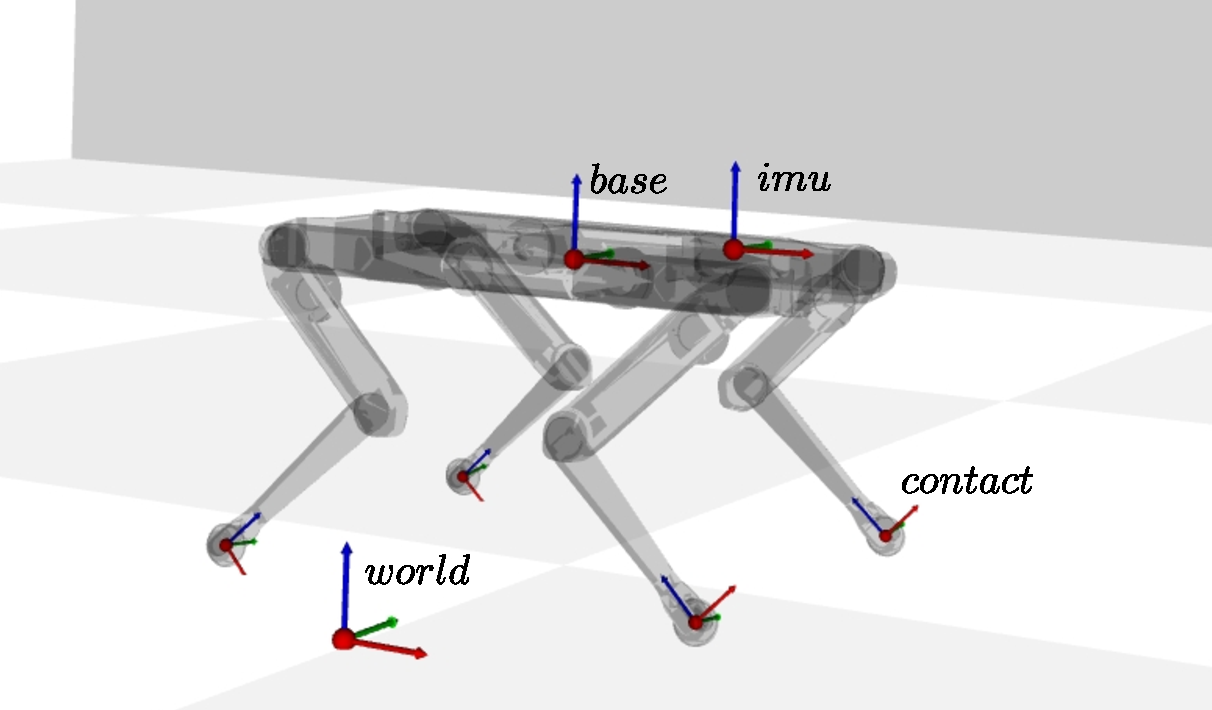
\includegraphics[width=0.6\textwidth]{figures/solo_frames.pdf}
    \caption{Solo 12 \cite{grimminger2020open} important reference frames}
\end{figure}
    

%%%%%%%%%%
\section{Proprioceptive base estimation}

We refer to proprioceptive base estimation for any state observer purely relying on proprioceptive sensors to estimate base frame states. 
The goal is then to design observers fusing IMU, kinematics, and possibly strain gauges measurements to obtain an odometry and orientation of 
the robot with respect to the gravity vector. The robot is akin to a blindfolded animal that has to balance and perform locomotion using 
only its inner ear, kinesthesis and sense of touch. \cite{bloesch2013state,rotella2014state} showed through an observability analysis 
that the absolute velocity, pitch, and roll angles as well as IMU biases are observable using only IMU and kinematic measurements when at 
least one contact is kept with the ground.

The roboticist has to make many design choices when building such a system. Those choices mainly include the way kinematic information is used in the system, 
the nature of the filter used (tightly-coupled vs loosely-coupled), how to detect stable contacts and whether extra sensors or more complex modeling need 
to be used to mitigate model errors.
 

\subsection{Kinematic information}
Legged robots move by interacting with their environment through intermittent contacts.
Once a stable contact (no slipping/tipping) is detected, the relative pose and velocity of the base with respect to the end-effector in contact 
can be computed through forward kinematics. Integrated over time, the relative displacement of the base of the robot can be inferred, a computation 
often referred to as \textit{leg odometry} (by analogy with wheel odometry). This computation takes about 1 microsecond thanks to libraries such as \cite{carpentier2019pinocchio, hereid2017frost}. It uses
readings from the joint encoders as well as the robot kinematic model. In systems with actuator reduction steps, encoders are usually placed before the reduction step 
to increase (... for solo \cite{grimminger2020open}). Joint velocities are often less precise since they are generally computed from numerical differentiation \cite{rotella2016imu}. 
The main sources of uncertainty usually come from inaccuracies in the parameters of the kinematic models such as approximate segment lengths, segments flexibilities \cite{vigne2018estimation}, 
joint backlash \cite{fallon2014drift} and flexibilities \cite{koolen2016design}. 
Bloesch \cite{bloesch2018technical} classifies kinematic measurement models in three categories that define the structure of this section. 
Those measurement models are summarized in \figRef{fig:kin_models}.


\textit{Feet matching} is the earliest example of leg odometry to be used in the leg robotics literature. Pioneered by \cite{roston1991dead} 
\footnote{An earlier example might exist in \cite{waldron1986adaptive} even though the technical report is unclear about the method they used: 
"Leg-position feedback is used from legs in support phase for the purpose of correcting for gyro and integration drift in the inertial reference system."},
multiple feet matching provides a relative 6D pose between moments during which at least three feet are in stable contact with the ground.
For point-feet robots (such as most quadrupeds, if their feet are sufficiently small to avoid rolling on the contact surface), the problem is an instance of the orthogonal Procrustes problem \cite{eggert1997estimating}.
Follow up works adapted the method to smaller hexapods \cite{lin2005leg} and began to fuse it with other sensors such as GPS \cite{gassmann2005localization, cobano2008location} 
and most importantly IMUs \cite{lin2006sensor, reinstein2011dead}.
The inherent limitation of this method is that for point-feet robots it requires at least three feet to be in contact with the ground between given timesteps, limiting
applications to hexapods (or more feet) or very slow quadrupeds gaits.
\textit{Single foot matching} is also possible for humanoid robots as each flat foot contact defines a 6D constraint \cite{bloesch2018technical}. 
After fixing the position of the contact by computing forward kinematics at the beginning of the stance phase, using the current base estimate, this constraint directly produces 6D 
relative displacements \cite{flayols2017experimental,xinjilefu2014decoupled,johnson2015team}. This approach is less investigated for point-feet robots and was first 
demonstrated (to the best of our knowledge) in my work \cite{fourmy2021contact}. Another work published later this year \cite{kim2021legged} also includes this 
factor formulation along with a null velocity factor. 

\textit{Instantaneous relative pose} between the base and the foot can also be directly used as a residual in the estimator. This formulation
was introduced in \cite{bloesch2013state, bloesch2013stateSlippery} for a point-feet quadruped using only relative positions. It was subsequently 
adapted for a humanoid robot \cite{rotella2014state}, whose 6D foot constraint permitted to add orientation information. In this formulation, 
states variables corresponding to the robot feet pose have to 
be added to the estimator. This approach was adopted by several other groups \cite{hartley2018legged, hartley2018hybrid, hartley2020contact, bledt2018cheetah}.
Potential undetected slips and rolls of the foot are modelled in this context as a random walk on stance foot position \cite{bloesch2013state,rotella2014state}. When the estimator is formulated as a 
\KalmanF \cite{kalman1960new}, this phenomenon is represented by a process noise on the feet position dynamics, which is a crucial parameter that the user needs to tune.

When a single point foot is in contact with the ground, the leg can move around the three remaining rotational degrees of freedom without changing encoder measurements.
The base \textit{relative velocity} can however be computed by using joint velocities and the angular velocity of the robot body. 
Joint velocities are usually obtained through numerical differentiation of the joint encoder outputs, which may result in noisy measurements \cite{rotella2016imu}.
Gyro measurements are also subject to noise and affected by a bias that should be compensated for. These velocity measurements can then directly be used as
residuals for the base velocity \cite{bloesch2013stateSlippery,bledt2018cheetah} or integrated over time as relative 
displacements \cite{ma2012robust, wisth2020preintegrated}. Some authors such as \cite{bloesch2013stateSlippery, bledt2018cheetah} 
use these types of measurements in conjunction with \textit{instantaneous relative pose} which seems to reduce position drift. On the other end,
one may argue \cite{fallon2014drift} that in the case of an erroneous kinematic model (backlash, flexibilities), using exclusively direct velocity measurements
prevents the estimator to become inconsistent when another source of position measurement is present (such as LIDAR localization). 

% CONLU
% Nicola's mini conclu -> more about the loosely/tightly-coupled dichotomy
% The methods listed here are the basis of most legged robot estimators, and we will use a similar structure in our work. Many different details are 
% considered, with various impact on the performances. In general, the reported works are difficult to directly extend die to the simplicity of the 
% estimator formulation and the lack of possibility to merge additional information. One of the ambition of my work is to keep the spirit and
% versatility of these estimators while enlarging the field of potentiality by using a nonlinear motion estimator.

These measurement models are the base of all legged robot estimators. We will see in the next section how they can be used with other data sources, 
in particular IMUs, to derive proprioceptive filters.



%%%%%%%%%%%%%%%%%%%%%%%%
% many "%" symbols used to avoid extra space added by latex compiler
% see https://tex.stackexchange.com/questions/42968/reduction-of-space-between-two-sub-figures
%%%%%%%%%%%%%%%%%%%%%%%%
\begin{figure}
    \centering
    \begin{subfigure}{.33\linewidth}
        \label{fig:kin_point_matching}
        \centering
        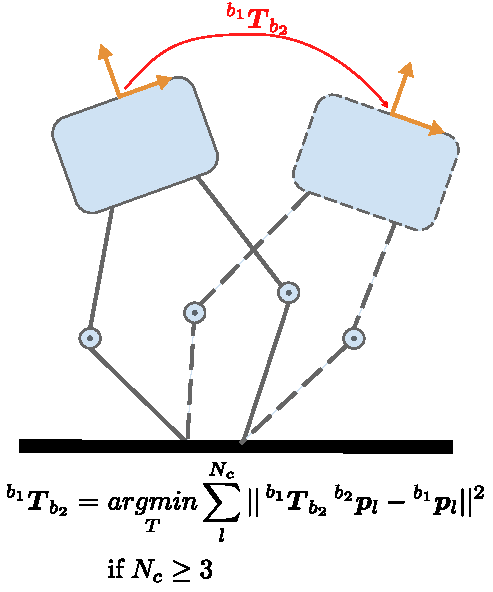
\includegraphics[width=\textwidth]{figures/robot_kinematic_types_point_matching.pdf}
        \caption{point-feet matching}
    \end{subfigure}%
    \hfill
    \begin{subfigure}{.33\linewidth}
        \label{fig:kin_point_direct}
        \centering
        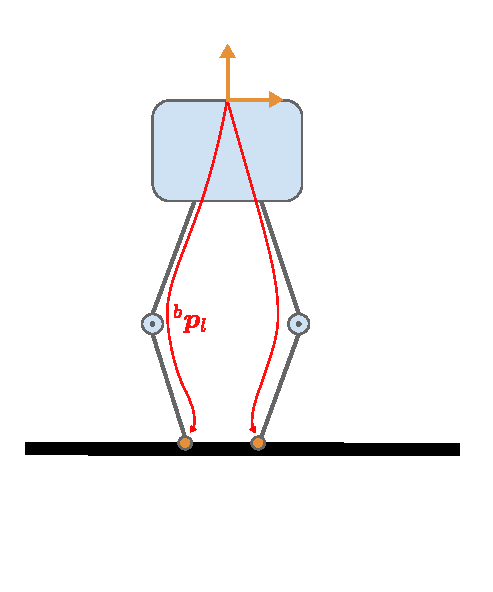
\includegraphics[width=\textwidth]{figures/robot_kinematic_types_point_direct.pdf}
        \caption{point-feet direct}
    \end{subfigure}%
        \hfill
    \begin{subfigure}{.33\linewidth}
        \label{fig:kin_point_vel}
        \centering
        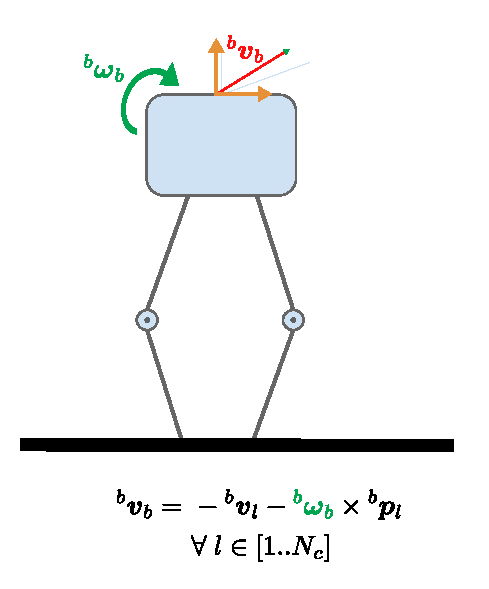
\includegraphics[width=\textwidth]{figures/robot_kinematic_types_point_vel.pdf}
        \caption{point-feet linear velocity}
    \end{subfigure}%

    \bigskip
    \begin{subfigure}{.33\linewidth}
        \label{fig:kin_flat_matching}
        \centering
        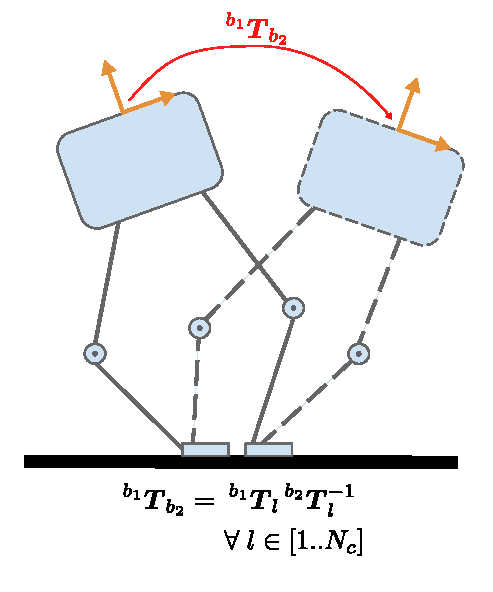
\includegraphics[width=\textwidth]{figures/robot_kinematic_types_flat_matching.pdf}
        \caption{Flat feet matching}
    \end{subfigure}%
    \hfill
    \begin{subfigure}{.33\linewidth}
        \label{fig:kin_flat_direct}
        \centering
        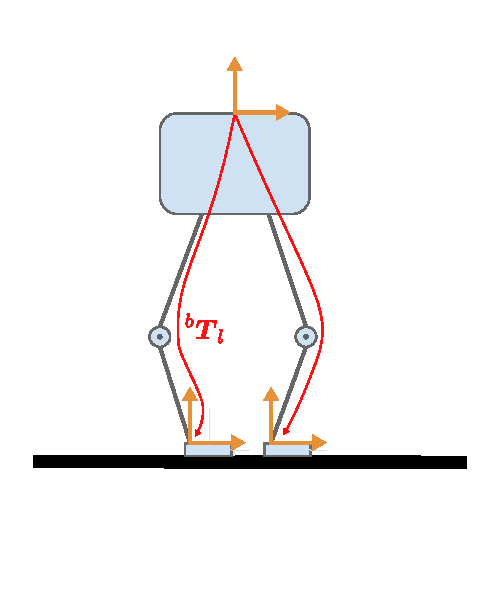
\includegraphics[width=\textwidth]{figures/robot_kinematic_types_flat_direct.pdf}
        \caption{Flat feet direct}
    \end{subfigure}%
        \hfill
    \begin{subfigure}{.33\linewidth}
        \label{fig:kin_flat_vel}
        \centering
        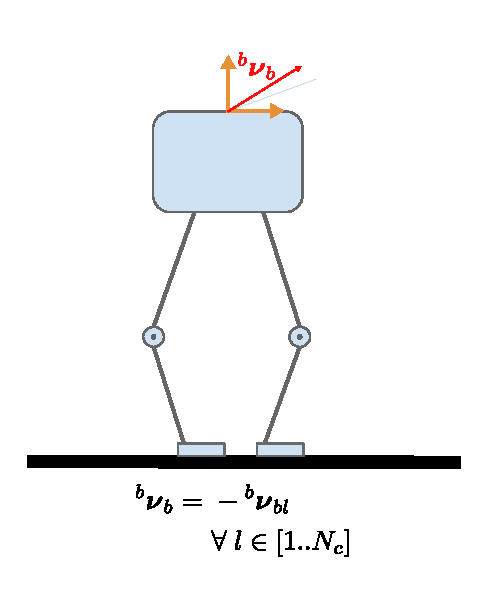
\includegraphics[width=\textwidth]{figures/robot_kinematic_types_flat_vel.pdf}
        \caption{Flat feet twist}
    \end{subfigure}%
    %
    \caption{Legged robots kinematic measurement models classification. Red arrows are used for the residuals derived for each model using encoder measurements and contact information. 
    orange elements correspond to the state variables affected by these residuals. Figures (\subref{fig:kin_point_matching}),(\subref{fig:kin_point_direct}),(\subref{fig:kin_point_vel}) are models
    for point feet robot, a model commonly used for quadrupeds. Figures (\subref{fig:kin_flat_matching}),(\subref{fig:kin_flat_direct}),(\subref{fig:kin_flat_vel}) are flat feet based models,
    commonly used for humanoid robots. The green rotational arrow represents gyroscope measurements that used in addition to encoders for the point-feet linear velocity model (\subref{fig:kin_point_vel}).
        }
    \label{fig:kin_models}
\end{figure}


\subsection{Filter based data fusion}
\label{sec:proprio_filters}

Many types of observer designs have been put to test on legged robots proprioceptive estimation. The problem being Markovian in nature,
most are continuous Bayes filters such as variants of the \KalmanF \cite{kalman1960new} and complementary filters \cite{higgins1975comparison}. While a complete history of 
the evolution of proprioceptive filters is instructive 
\cite{gassmann2005localization, lin2005leg, lin2006sensor, cobano2008location, aoustin2008experimental, lebastard2011estimation, chilian2011multisensor, reinstein2011dead, 
gur2012model, ma2012robust, gorner2013leg}, 
this has been treated exhaustively by other authors \cite{bloesch2017state, camurri2017multisensory}. 
It is however interesting to delve into a particular dichotomy between different estimators implemented in recent works. Those can be 
roughly divided between \textit{loosely-coupled} (LC) approaches, which divide the estimation in several steps whose results are being successively taken as fixed priors to the 
following steps and \textit{tightly-coupled} (TC) approaches, which try to capture all statistical cross-correlations between the estimated states.

In the context of proprioceptive estimation, a common loosely-coupled filter is to pre-compute the base orientation independently by a first filter and using it as a fixed value in subsequent filters. For instance, during the 2015 DARPA robotic challenge, the CMU \cite{feng2015optimization} and IHMC 
\cite{johnson2015team} teams explain that they implemented tightly-coupled nonlinear estimators for the early trials, based on ad hoc 
implementations of proprioceptive filter, but ended up using the orientation estimation provided by the ATLAS IMU without modification later in the competition preparation.
This was helped by the fact that ATLAS IMU was a tactical-grade fiber-optic model. 
An experimental comparison of two decoupled proprioceptive filters for \HRP{2} was proposed \cite{flayols2017experimental}. For both, a complementary filter estimates 
the orientation of the base from IMU measurements only. The second step is either a straightforward \KalmanF on the position and velocity or an ad hoc two-stage 
weighting algorithm: first orientation weighting between the IMU and both feet, then position and velocity measurements 
weighting between both feet. Similar decoupled approaches have been implemented on quadruped robots such as a \KalmanF for \cite{bledt2018cheetah} and a two-stage complementary filter for \cite{leziart2021implementation}.

The \textit{tightly-coupled} approach to proprioceptive base estimation was first introduced in works like \cite{chilian2011multisensor}, but \cite{bloesch2013state} was the most decisive step.
In this work, states of interest (position, velocity, orientation, IMU biases) are jointly estimated in an error state \KalmanF (ErKF). Strapdown integration of an IMU and 
a direct kinematic model were used. In particular, translation-orientation coupling was showed to play a central role in making the IMU biases observable. 
An observability analysis and experiments showed that the orientation degrees of freedom need to be slightly excited to decipher accelerometer bias from the projection of the 
gravity vector. The same coupled approach was applied to humanoid robots \cite{rotella2014state, fallon2014drift}.
\cite{hartley2020contact, lin2021deep} take another step toward coupling the state variables by expressing the aforementioned variables as a single matrix Lie group.
This new kind of estimator called Invariant \KalmanF \cite{barrau2018invariant} exhibits a larger pool of convergence compared to the EKF and cannot become 
inconsistent because of linearization issues. 

All in all, one of the major factors affecting the choice in favor of either a tightly or loosely-coupled estimator is the quality of the platform sensors. Other factors may include personal experience of the designer, software/hardware architecture, need for modularity etc. 
A very high-end IMU such as the ATLAS fiber optics IMU will be able to compute a very consistent orientation and even biases inside its internal 
filter using an approximate motion model. On the other end, a lower quality IMU may require data fusion from sources such as leg odometry, 
provided that this source of information is not too biased. Progress in miniaturization and production of MEMS-based IMUs, which equip most 
legged robots nowadays, seem to guide to the use of staged approaches for quadruped robots \cite{bledt2018cheetah, leziart2021implementation}. 
However, these IMU classes still represent a significant portion of the robot's price. Furthermore, we believe that, in the long-range, tightly-coupled
approaches present several advantages. Firstly, as legged robot gains in industrial maturity, TC carries the promise of augmented performances by being able
to more easily integrate online debiasing and calibration of lesser cost sensors. Secondly, as a software tool, we will show in this thesis that libraries based
around tightly-coupled estimators may enable more versatility in the observer design. However, as we will see in \secRef{sec:sota_factor_graph} 
tightly-coupled estimators implementations based on Bayes filters do not scale up well to use exteroceptive sensors, which motivate us to use in our work of a
new class of estimators, based on factor graph optimization.

% MIT cheetah: KVH Industries 1750 -> ?$
% Solo12:   2k$


\subsection{Contact detection}
As we saw, a critical part of legged robot estimation is the integration of kinematic information when feet are in contact. A major
assumption of those methods is that the stable contacts are known a priori. The definition of a stable contact depends on the system: for quadruped that 
are usually equipped with point-feet, three positional degrees of freedom are blocked, the leg only being able to rotate around the contact point; 
while for a humanoid robot with planar feet, the six degrees of freedom are constrained. Slipping appears when the contact forces go outside of the Coulomb friction cone, 
that is when the ratio $f_{\parallel}/f_{\perp}$ (where $f_{\parallel}$ and $f_{\perp}$ correspond to the tangential and normal components of the contact force) 
exceeds a certain threshold, called friction coefficient. 
This coefficient is generally unknown as it depends on the nature of the foot and ground surface properties.

The most generally available information is the planned sequence of contacts \cite{bledt2018contact}, which may be assumed to be approximately respected in nominal operation. 
While relying only on a prior plan lacks robustness due to unexpected events such as changes in terrain heights and feet slips, is straightforward to implement and 
does not require extra sensors. Some robustness can be gained by reducing the confidence in the contact soon after impact or just before takeoff. 
\cite{leziart2021implementation, bledt2018contact}. Most high-end humanoid robots however \cite{stasse2017talos, englsberger2014overview} are 
equipped with strain gauges at their feet that can fairly accurately measure the ground reaction forces (GRFs). 
Though often biased depending on temperature, force measurements can be used as a proxy to stable contact by setting a reasonably large threshold \cite{fallon2014drift}. 
This method is an approximation of checking the Coulomb cone.
However, for quadruped slip detection, Focchi \cite{Focchi2015SlipDA} argues that force sensing is not enough, because the friction coefficient,
as well as the contact normal, is generally hard to infer. The authors propose a simple algorithm checking relative feet velocities values in the base frame and discarding those
far from the median. A similar choice is made by \cite{bloesch2013stateSlippery} in which Unscented \KalmanF velocity updates are rejected as outliers if their innovation exceeds a threshold.  
More recent papers try to fuse these different sources of information in Bayes filters. \cite{hwangbo2016probabilistic} and subsequently \cite{jenelten2019dynamic} fuse 
the kinodynamic models of the robot, IMU measurements, joint encoders values (and their first and second-order differentiation) as well as
joint torques in a discrete Hidden Markov Model (HMM) where contact states are binary values. A HMM is used instead of a continuous Bayes filter because the feet state are modeled as taking a finite set of values: either in contact or not.
They build separate filters for contact and slip detections and demonstrate walking on ice with an 
\mbox{ANYmal-C} using a special controller. A similar approach formulated as a \KalmanF directly estimates contact probabilities \cite{bledt2018contact}. 
It questions previous works that assume the availability  \cite{hwangbo2016probabilistic} or negligibility \cite{camurri2017probabilistic} of joint angular 
accelerations in the context of whole-body dynamics end-effector force estimation.
It proposes to instead rely on a new formulation of the \textit{generalized momentum} estimator to estimate forces based on first-order derivative only by exploiting the 
structure of the whole-body dynamics Coriolis matrix. The gait cycle is taken into account as a process model and is fused with kinematics and contact forces updates.  

This problem is not trivial and practical solutions seem to hesitate between simple heuristics and complicated Bayes filters. 
The problem with simple heuristics is that they neglect the temporal aspect of the data stream. On top of that, their parameters (though few in numbers) may be hard to tune.
Bayes filters, on the other hand, provide more fine-tuned control of the modeled aspects of the problem, at the expense of complex parameter tuning.
One thread of research tries to alleviate the need for tuning by relying on data-driven approaches. Supervised learning can be used \cite{camurri2017probabilistic} 
to introduce a probabilistic contact detector using only joint torques and robot kinematics, expressed as a logistic regression. 
The detectors provide a probability distribution on feet contacts that is used to ponder kinematic measurements of an tightly-coupled proprioceptive filter. 
The method outperforms a baseline based on threshold selection. However, the method %seems to require manual annotation of datasets and 
fits different thresholds for each type of gait and may certainly suffer from different terrains and robot loads. 
Rotella \cite{rotella2018unsupervised} proposes to cluster fuzzy contact states by training an unsupervised model on humanoid robot simulated data. The datasets are augmented
with IMU measurements at the feet that are removed at evaluation time. The resulting estimator odometry system is shown to outperform a contact force classifier
but was not validated on real hardware. More recently, Lin \cite{lin2021deep} proposed to train a deep neural network to infer contact states using a buffer of 150ms of raw IMU, 
encoder, and kinematic measurements. The emphasis is put on training the estimator in various ground types in outdoors extended environment using an MIT Mini Cheetah. Ground truth is generated
by finding a region around the local minimum of low passed feet height trajectories in the hip frames. The estimator provides a reliable source of contact information 
and generalizes better to different environments. It does not provide covariances about the contacts, contrary to \cite{camurri2017probabilistic}.  

% CONLU
Contact estimation is a still burgeoning field of research, especially for small quadrupeds which often do not embed contact sensors. The main reason 
is the fact that adding extra weight at the very end of the legs can increase significantly the leg's inertia, limiting the explosivity of possible movement. The 
extra electronics and wiring required may also be a limiting factor.  


\subsection{Kinematic model inaccuracies mitigation}
% BAD
% Only high-end IMUs measurements can be reasonably used directly without somehow taking biases into account.
% Similarly, for some robotic system, forward kinematic can suffer from encoder noise and kinematic model biases. Some authors propose to 
% augment the capabilities of their estimator by adding extra sensor modalities or directly modeling the model inaccuracies (mainly flexibilities).

% Nicolas', but not very appropriates since not "bias" estimation here
% As explained in \secRef{sec:def}, IMU measurements are intrinsically biased. On high-end IMUs, often used in lab prototypes, this bias is either 
% reduced by high-quality hardware or compensated by the integrated electronics, and can be neglected. Yet this bias must be taken into account, ie.
% estimated and compensated, for more general setups.
% In general, biases cannot be estimated from the only sensor measurements. We then say that the biases are \textit{observable} for the sensors alone (?). 
% Additional information, either from physical models assumptions or external measurements, must be added to the filter to make the biases and the states observable
% together.

% New one
We have seen in \secRef{sec:proprio_filters} that most legged robot proprioceptive filters rely on the robot kinematics in order to bound the drift of the integration
of the inertial odometry and debias IMU raw measurements. However, to obtain consistent filters, special care has to be taken to ensure that the kinematic
measurements are not themselves biased. Mainly two main issues have been identified and addressed so far in the literature: inaccuracies in the joint velocities derived from
encoder measurements and the undesired flexibilities of robot segments and joints.

Encoders measuring joint angles are usually placed at the actuator level \cite{xinjilefu2014decoupled}. 
They produce a very precise angle estimation when subsequent reduction steps are present. It is then acceptable to numerically 
differentiate and slightly filter those values to use them for joint impedance control for instance. However, hydraulic
actuators do not include such reduction steps and fall victim to important joint velocity noise, which can degrade feedback control.
Xinjilefu \cite{xinjilefu2014decoupled} proposes to use the dynamic model of the robot and joint torques to obtain filters on the joint angles and velocities
of the ATLAS robot. The same author \cite{xinjilefu2016distributed} also implemented a network of low-cost gyroscopes to estimate the joint velocities 
on the same platform. A \KalmanF is used to fuse desired joint acceleration from the control as process input and angular velocity measurements coming from 
the MEMS and numerical differentiation of the encoders. It requires a calibration procedure of the gyroscopes orientations and a good quality attitude
estimation of the base, from a high-grade IMU for instance. This method was extended in \cite{rotella2016imu} by also including
accelerometers measurements, explicitly compensating IMU biases, and alleviating the need for a global attitude estimation.

Another source of kinematic error comes from the presence of flexibilities in the structure of the robot, which is a common problem in many human-sized legged robots. 
For the \HRP{2} humanoid robot, a rubber joint is placed at the ankle to mechanically absorb feet impacts. 
It also acts as a rotational spring that, given the length of the ankle-base lever, 
leads to important and unmeasured base accelerations. \HRP{2} being equipped with 6 axis 
force sensors at the end-effectors, \cite{flayols2017experimental} proposes to map these measurements to relative orientations that can 
directly be included in the kinematic chain as an intermediate ball joint. Calibration of the stiffness matrix is done by comparing 
kinematics to motion capture measurements. \cite{benallegue2015estimation} derives a procedure to alleviate the need for force sensors by 
designing a centroidal filter using an inverted pendulum dynamical
model. For the Wandercraft exoskeleton \cite{harib2018feedback}, flexibilities
are shown to be spread along the successive segments of the kinematic chain, and can be modeled as punctual, 
3d rotations with a linear spring behavior \cite{vigne2018estimation}. This work implements an IMU network similar to the ideas of 
\cite{xinjilefu2016distributed,rotella2016imu} but it uses independent complementary filters for each IMU to recover their absolute orientation. 
These orientations are then used as virtual joints and fused with the robot whole-body dynamics and the linear spring models to recover segments 
relative orientation and angular velocities.

Other kinematic uncertainties are however often present and are harder to model or sense. For instance, the foot of the quadruped used in 
\cite{bloesch2013state} is spherical but is only modeled as a point. Backlash prevented Fallon \cite{fallon2014drift} to use a direct kinematic 
measurement model and was one of the limiting factors of Vigne \cite{vigne2018estimation} estimator.
These works advocate for the addition of many different sensor sources in the estimator, in particular to account for the limited observability
capabilities of legged systems and to benefit from cheap, distributed, low consumption sensors. Ideally, we could see the evolution of legged
robot estimation going toward whole-body perception. In our opinion, the main limiting factor to that goal is the mathematical formulation of efficient tightly
coupled estimators, to which this thesis would like to contribute.  


%%%%%%%%%%
\section{Dynamic centroidal estimation}
%
\subsection{Why is centroidal dynamic estimation important?}
Legged robots are highly nonlinear systems that use contact forces between their end-effector and the environment to implement stable locomotion. 
The effect of these forces is dictated by the Newton/Euler equations, also known as the underactuated dynamics, which state that the variation of the 
system momentum is equal to the external wrench applied to the robot. Though these equations may appear simple, they introduce a nonlinear coupling 
between the CoM position and the angular momentum. Many reduced-order models are based directly on 
various levels of approximation of these equations \cite{kajita20013d, wieber2006trajectory, carpentier2016versatile} to derive predictive
control algorithm, for locomotion for instance. These works assume knowledge of centroidal quantities of the system at control frequency, 
namely the position of the center of mass, angular momentum, and their derivatives. 
It is therefore crucial to implement accurate and efficient estimators for these quantities.

\subsection{Information sources}
Assuming that the base state and joint configurations are perfectly known (up to linear and angular accelerations), it is theoretically possible 
to compute all centroidal quantities using the kinematic model of the robot and the distribution of mass in the different segments. 
However, this model is most often obtained from CAD data that may be inaccurate. This may call for a calibration of
the platform \cite{ayusawa2008identification, ayusawa2014identifiability, bonnet2018inertial, bonnet2019overview}. 
This problem was closely scrutinized in the biomechanics literature where mass distributions often come from standardized anthropomorphic tables \cite{de1996adjustments}. 
A second kind of information comes from measurements of the external wrench. 
Forces provide the CoM accelerations while moments relate to the CoM position through a line called the central axis. This line passes only approximately by
the CoM because of gesticulation \cite{wieber2000modelisation} induced angular momentum variations \cite{wieber2006holonomy}. Moreover, the wrench measurements 
are usually noisy and require the presence of expensive deformation gauge sensors at each contact point. A complete analysis of the particularities
of these different information sources along with an observability analysis can be found in \cite{carpentier2016center}. 
This fosters the use of more complex algorithms by fusing kinematic and external wrench measurements. 

\subsection{Reduced dynamical models}
The contact wrench is not always directly accessible to the estimator. For instance, the Atlas robot gauge sensors measure only the contact normal force
and horizontal moments. Thus, the exact underactuated dynamics cannot be directly used. Some works propose to use simplified models of the 
dynamics that require less information. For instance, the popular Linear Inverse Pendulum Model (LIPM) \cite{kajita20013d} treats the body as a lumped mass, 
centered at the center of mass (COM), that only moves horizontally and therefore neglects the robot angular momentum. It only requires the position of the 
Center of Pressure (CoP) to obtain the CoM dynamics. The CoP is defined as the point where the moment component of the resulting wrench is aligned with the normal 
axis of the plane. The computation of this point only requires the contact normal force and horizontal moments, which is coincidingly the kind of
sensor present on the Atlas robot.

Stephens \cite{stephens2011state} proposes to use the LIPM for the process model to an EKF 
that also includes kinematic measurements. Model errors in the form of a CoM position measurement 
offset and external forces are added to the formulation and it is shown that either of these quantities is observable. 
Xinjilefu \cite{atkeson2012state} ponders the use of a more complete planar sagital dynamical model by comparing it to the LIPM model
without introducing model biases as was done in Stephens \cite{stephens2011state}. It instead relies on tuning filter covariances to alleviate their effects. 
Simulation shows that the LIPM seems more able to cope with model errors but performances on the real robot show similar results. 
One of the benefits of this model is that force measurements can be summarized by the Center of Pressure (CoP) (aka. Zero Moment Point (ZMP) \cite{sardain2004forces}).
In the context of Darpa robotic challenge, the CMU team later implemented a centroidal estimator \cite{xinjilefu2015center} similar to that of Stephen \cite{stephens2011state} that was able to prevent a fall during the challenge finals. 
Similar EKF based estimators using respectively a LIPM \cite{piperakis2016non} or a fly-wheel process model \cite{piperakis2018nonlinear}, which models a non-zero angular momentum contrary to the LIPM,  is later implemented on a NAO robot. 
Because the robot used for the experiments is equipped with a single axis ground reaction sensor,
the process model has to be used again in the measurement model equations.   
A LIPM process can also be used with a fixed contact point assumption \cite{benallegue2015estimation}. By a tight fusion with IMU 
measurements and kinematic information, centroidal quantities can jointly be estimated with joint flexibilities at the ankles under external force disturbances. 
The particularity of this approach is to avoid the need for force sensors but it is restricted to motions with fixed rigid contacts with the ground 
such as during manipulation.
Xinjilefu \cite{xinjilefu2014dynamic} took a different approach by estimating unmeasured components of the feet contact wrench (only normal force and pitch+roll torque are measured)
This was done by leveraging the whole-body dynamics of the humanoid robot, IMU, and kinematic measurements. 
A generalized torque slack variable was introduced to represent the dynamical model errors. %External wrench at the feet is also a state variable as the measurement model on this quantity is only partial. 
The estimator was formulated as a QP using this generic formulation which permits to enforce inequality constraints on state variables. 
It is used to model joint limits and the positivity of normal ground reaction forces (the robot can only push on the ground).


\subsection{Estimators based on underactuaded dynamics}
While previously mentioned works rely on approximate dynamical models, we must acknowledge that an inaccurate process model must lead to a biased estimation. 
Rotella \cite{rotella2015humanoid} proposes instead to use the underactuated dynamics. 
The authors build several estimators by fusing six-axis force/torque sensors and kinematic measurements in an EKF. 
These estimators introduce offsets on CoM position and linear momentum as well as an external 6D wrench disturbance. A nonlinear observability analysis is conducted 
and shows that either the biases or the external wrench are observable. 
Carpentier \cite{carpentier2016center} chooses a different viewpoint by proposing a frequency analysis of the information sources used for centroidal estimation. The model
assumes the presence of wrench sensors at the contacts and does not require explicit modelling of the kinematic bias and external disturbances. Instead, it relies on a complementary filter
to filter out problematic frequency bands in each signal. For instance, kinematic measurements are high passed filtered to remove its slowly varying bias. 
Bailly \cite{bailly2019recursive} extends this methodology to include CoM acceleration and angular momentum derivative in the estimation variables. Both works showed to outperform
a simple EKF by offering an unbiased CoM position estimate.
The same author \cite{bailly2021optimal} propose to use Differential Dynamic Programming (DDP), an algorithm traditionally used as a Optimal Control Problem solver \cite{mastalli2020crocoddyl}.
This algorithm estimates the same quantities as the previous work of the author \cite{bailly2019recursive} by solving a Maximum A Posteriori (MAP) problem on a sliding window of states sampled at IMU frequency, 
which permits to back-propagate information from the future to the past. The approach compares favorably to both previous work \cite{bailly2019recursive} and a simple EKF.

% CONCLU



%%%%%%%%%%
\section{Environment awareness}
Any useful task undertaken by an autonomous robot involves some level of awareness of its environment, even for partially teleoperated robots \cite{koolen2016design}. 
For ground robots, this problem is most often tackled with exteroceptive sensors such as cameras, depth cameras, and LIDARs.
The environment might be known through a previous mapping procedure like Structure from Motion (SfM) \cite{triggs1999bundle} or mapped on the fly. 
Applications can be such as localizing with respect to a known map \cite{dellaert1999monte},
following a previously traversed path without a metric map \cite{furgale2010visual}, Simultaneous Localization And Mapping \cite{aulinas2008slam, cadena2016past}, object detection and pose retrieval \cite{du2021vision}, 
autonomous exploration \cite{rouvcek2019darpa, kulkarni2021autonomous}... An intermediate case is the one of visual/LIDAR odometry in which a local representation of the environment is built to provide a precise odometry source \cite{scaramuzza2011visual} and is later discarded. 

% Dense semantic mapping
\cite{gan2020bayesian}


The particularity of legged platforms is that they interact through intermittent contacts to move, usually using predefined cyclic gaits. While some controllers are 
robust enough so that a purely proprioceptive estimation provides enough feedback even in complex environments \cite{tan2018sim, lee2020learning}, having an estimate of 
the terrain shape may help planning steps. Moreover, multicontact approaches \cite{carpentier2017multi, henze2017multi} in which arms of a humanoid may also be used 
for locomotion are a promising way to increase the range of possible movements and reduce energy consumption. 

The literature related to these questions is immensely vast and goes largely beyond the scope of this thesis, although the formal underlying methods are closely related,
as we will see in \secRef{sec:sota_factor_graph}. Moreover, we will see that our ambition and latest results tend to merge legged estate estimation with
exteroceptive localization and mapping at large. We will quickly review the most relevant works, first focusing on localization eg. for navigation, then 
on dense mapping for contact planning. 

\subsection{Localization and mapping}
IMU/kinematics fusion inherently drifts in position and yaw orientation. For teleoperated tasks, this drift may not be problematic as the balance control loop
mainly requires instantaneous base velocity and orientation with regard to the gravity while navigation can be handled by the operator. However, for autonomous
navigation, it becomes critical to have some kind of precise odometry or localization strategy, or, even better, being able to run onboard Simultaneous Localization And Mapping. 
\cite{davison2007monoslam} is the first example of a monocular vision-based SLAM system implemented for the navigation of a humanoid robot \HRP{2}. The gyro of the robot
is also incorporated in the filter at the camera rate to minimize the growth of uncertainty before loop closing. \cite{stasse2006real} expends on this concept by also fusing
kinematic velocity and altitude (known from the planning). Other systems based on sparse features were later developd \cite{ahn2012board, oriolo2012vision, oriolo2016humanoid, kwak20093d}. 
Visual Teach and Repeat \cite{furgale2010visual} has also been recently brought to quadruped 
robots \cite{mattamala2021learning}, which opens up practical long-term operations in industrial environments. Some works also propose to use mature visual odometry libraries
as black-boxes sources of odometry by integrating them as relative pose measurements \cite{hartley2018legged,hartley2018hybrid}. While it may lead to sub-optimal estimators, 
this method has the benefit of greatly simplifying the development process.

While a camera system benefits from low-cost and hardware integration difficulty, outdoors environments 
may cause some difficulties to such systems, such as shadows being mistaken for solid edges (Figure 8. of \cite{fallon2014drift}).
During the 2015 DARPA robotic challenge, where robots had to semi-autonomously traverse challenging environments while performing manipulation tasks at known given checkpoints,  
LIDAR information was crucial for teleoperated manipulation tasks \cite{koolen2016design} which required a precise metric representation of the scene. 
Localization with respect to a fixed map also proposed \cite{fallon2014drift} but not used in the finals \cite{fallon2016perception}. In fact, though supposed 
to represent a closed static industrial environment, the final trials happened in a semi-opened outside place with an important moving crowd on one side, making
LIDAR localization very noisy. 

\cite{hornung2014monte} proposed to apply Monte Carlo Localization using LIDAR measurements by using a highly efficient global Octomap data structure \cite{hornung2013octomap}.
The algorithm is validated on a NAO humanoid robot and used a learned leg odometry motion model, pitch and roll information from the IMU as well as an edge-based vision measurement model.
The MIT team \cite{fallon2014drift} uses the same method but replaced the motion model with an inertial kinematics proprioceptive filter. 

LIDAR can also be used as an odometry source by matching point clouds taken at successive timestamps with ICP. However, this procedure is time-consuming 
and leads to time delays with respect to other measurement sources, which is generally a problem for Bayes filters. 
Nobili \cite{nobili2017heterogeneous} solves this issue by keeping a buffer of past belief state of the EKF, a method on which is 
based the Pronto framework \cite{camurri2020pronto}.

% CONCLU



\subsection{Reconstruction for footstep planning}
Even though some legged robots designs and controllers \cite{reher2019dynamic, bledt2018cheetah} are robust, to some extent, to terrain model uncertainty, having information about the local
shape of the environment enables a more reactive contact planning. For instance, the guide path implemented in contact planner \cite{tonneau2018efficient} uses the complete 3D structure of the environment
provided as an STL file while a mixed integer contact planner like \cite{tonneau2020sl1m} uses a list of vertex tuples representing convex planar surfaces.
Most reconstruction implementations rely on a depth sensor to obtain these representations.

An interesting representation is to build a grid-based \textit{elevation maps}, that associates a probabilistic distribution to the height of each 2D cell. 
This is a simplified representation of the 3D environment, that does not take terrain slopes into account for instance, but provides interesting computational features. 
For rover applications, one can argue that building a globally consistent elevation map is too costly and it is instead more efficient to switch the representation to 
the local robot frame \cite{kleiner2007real}. 
The map is constantly updated using two sources of information: range measurements that refine the visible parts of the map; wheel odometry that increases uncertainty on the map 
using heuristics based on the traveled distance. \cite{fankhauser2014robot, fankhauser2018probabilistic} adapted these ideas to legged robots. The map grid probabilistic representation
was also improved by including horizontal uncertainty due to the robot's relative motion. A costly map fusion process that computes lower and upper bound on the elevations
is decoupled from the sensor updates and can be computed intermittently at the discretion of the user. 

An extension of the elevation grid map is to represent occupied 3D space as an 3D occupancy voxel map, which can be efficiently stored using an Octomap.
While \cite{hornung2014monte, fallon2014drift} only used this representation as prior for online localization, it was used for online foot planning in \cite{winkler2015planning, mastalli2015line}. 

\cite{kolter2009stereo} adopts a mesh representation built from point-clouds aligned twice a second off-board using an ICP procedure initialized by proprioceptive odometry and filled with
a texture synthesis step. This representation directly provides richer information such as the slope of the terrain which is used in \cite{mastalli2020motion} to 
tightly couple motion/step planning and terrain reconstruction.

\cite{fallon2015continuous} used the Kintinuous framework \cite{whelan2012kintinuous} to obtain a local Truncated Signed Distance Function based dense representation. This map was
shown to be of equivalent quality to that of a LIDAR and used as an input to a feasible contact surface segmentation algorithm selecting planar convex regions of uneven cinder blocks. 
In order to handle local loopy trajectories better than Kintinuous, Elastic Fusion \cite{whelan2016elasticfusion}, which is a surfel-based dense depth vision system, 
was shown to be usable on humanoid platforms \cite{scona2017direct}. The system augmented the Elastic Fusion algorithm by adding 
proprioceptive odometry term to the solved least squares system, using a heuristic to increase the weight of proprioception in visually degenerate situations. The 
dense reconstruction is accurate up to 2cm, which is enough for motion planning. However, in this case, the map was only used for localization.

% CONCLU
Online terrain reconstruction extends the capabilities of legged robots to uneven surfaces. It is however not central to the problem statement of this thesis and is considered as
out of scope. Our main goal is to investigate a new class of estimators based on Factor Graph optimization, which we will now introduce. 


%%%%%%%%%%
\section{Factor Graph optimization}
\label{sec:sota_factor_graph}
As we have previously discussed, the largest part of the legged robotics state estimation literature consists in fusing sensor modalities using various 
implementations of the Bayesian and complementary filters. The core of those systems consists of a tightly or loosely-coupled IMU/kinematics proprioceptive
filter. Then, either this proprioception is used as a prior odometry source to a SLAM system or the exteroceptive sensors are used to localize with respect to a known map,
making position and yaw observable.

A different kind of estimator has been investigated over the last decades in the visual/LIDAR SLAM community and has become predominant in applications
such as drone navigation: \textit{factor graph optimization}, also known as simply \textit{graph optimization}. 
While the Bayes filter summarizes  the accumulated information about the current estimated state and its cross-correlations as a single probabilistic distribution, 
Factor Graph optimization keeps a trajectory of arbitrarily spaced past states that are regularly re-optimized in the least square sense, by finding the so-called 
Maximum A Posteriori over the trajectory joint distribution. The terms smoothing and mapping or sliding window estimator are also used when a limited window of past states are kept 
in the estimator, the old ones being marginalized. The earliest example \cite{lu1997globally} proposed to obtain globally consistent 2D LIDAR range 
scan alignments by minimizing a cost function over a trajectory of 2D poses constrained by LIDAR scans and wheel odometry.
 Many ad hoc efficient solvers such as \cite{grisetti2011g2o, dellaert2012factor, ila2017slam++, ceres-solver} have been developed 
over the years to leverage the specific sparsity of the SLAM problem.

While the first successful online monocular visual SLAM algorithm was implemented using an EKF \cite{davison2007monoslam}, a breakthrough happened with the 
Parallel Tracking And Mapping (PTAM) system \cite{klein2009parallel} that proposed to split the visual tracking of features and camera motion from the 
mapping in separate processes. This new modularity enabled the use of a specific algorithm for the mapping part: Bundle Adjustment \cite{triggs1999bundle} of sparse features, a method that was previously reserved for offline SfM 
pipelines . PTAM enabled Augmented Reality applications in limited spaces. Bundle Adjustment is actually a special case of a more general estimation algorithm called graph optimimzation which has several conceptual and computational advantages over filtering.
A great wealth of papers following both methodologies were subsequently published. A thorough comparison 
of the two approaches \cite{strasdat2012visual} concluded that the graph optimization was computationally superior in that it had the greatest precision to 
computational cost ratio, for most benchmarks. Most of the state-of-the-art visual SLAM framework now follow a factor graph approach 
\cite{forster2017-TRO, mur2015orb, qin2018vins, leutenegger2015keyframe, ferrera2021ov}.

\subsection{Very short intro intro to factor graphs}
...

Advantages of factor graphs: 
- tight coupled
- front/back end architecture allows modular design
- re-linearization allows to achive better accuracy than EKF-like
- sparse formulation allows very fast solving
- graph representation is intuitive and eases up the design of complex multi-sensor estimators


\subsection{Visual-Inertial odometry}
To robustify visual SLAM/odometry systems in cases of adverse situations, IMUs provide complementary high rate odometry information that can 
be debiased by tightly coupling mapping and odometry. A careful preintegration \cite{lupton-09,forster2017-TRO} of these high 
rate measurements had to be developed in the context of smoothing for the optimization to remain tractable. The core idea of this algorithm has 
since been applied to other information sources such as drone thrust commands \cite{nisar2019vimo} to make external force estimation possible.

\subsection{Factor Graph estimation for legged robots}
Very recently, two teams started to apply factor graph optimization principles as a general framework for legged robot estimation. At Michigan University, Hartley \cite{hartley2018legged} 
proposes to fuse IMU preintegration with a novel kinematic factor by adding the contact foot pose in the optimized states, similarly to \cite{bloesch2013state,rotella2014state}. 
Semi-direct Visual Odometry \cite{forster2014svo} is also used to integrate camera measurements as relative pose. The estimation framework was based on GTSAM framework \cite{dellaert2012factor}
and tests were conducted on a Cassie bipedal robot. In \cite{hartley2018hybrid}, the same authors extended 
modified the kinematic factor formulation, taking into account uncertainty induced by contact switches. Dynamic Robot Systems Group at Oxford proposed in 
\cite{wisth2019robust} to replace a modeled kinematic factor by integrating odometry from the onboard proprioceptive filter of the ANYmal robot. Stereo vision was also used as a source of
odometry by using a sparse 3D landmark map. In a following work \cite{wisth2020preintegrated}, the proprioceptive odometry factor was adapted
to include a slowly variable bias on odometry measurements by adapting the preintegration theory from \cite{forster2017-TRO}. They again extended this work
by including LIDAR measurements in \cite{wisth2021vilens}.
\cite{kim2021legged} also implemented an inertial kinematic proprioceptive smoothing estimator on the MIT Cheetah, mitigating slipping of the feet by removing kinematic 
measurements whose residual errors exceed a certain threshold.    


The maturity of the aforementioned factor graph optimization solver libraries certainly played an important role in these recent developments. It seems
that tools originally developed in the SLAM community are making their way in the legged robot community. Software libraries are becoming more
generalist, more precise and, based on Lie theory \cite{sola2018micro}, they handle more nicely the specificities of the manifold structure of the problem variables.
Other projects propose to deal with the inherent complexity of multi-sensory systems, proposing principled ways to handle multiple data sources, potentially asynchronous and at
different frequencies. Those frameworks also provide a mathematical formulation for most common sensor models and higher level interfaces with least-square solvers 
in an effort to bring these techniques to a broader audience \cite{sola2021wolf, blanco2019modular, colosi2020plug}.

